\documentclass{article}
\usepackage[utf8]{inputenc}
\usepackage{amsmath}
\usepackage{ dsfont }
\usepackage{graphicx}
\usepackage{array}


\title{Trabajo práctico de R}
\author{Kevin Frachtenberg, Ruslan Sanmartin Sobol , Celeste Rodriguez}
\date{27 Junio 2017}

\begin{document}

\maketitle

\section{Ejercicio 1}

$X_1,...,X_n =$ m.a. iid U[0,b]

1) $b_{mom}$: $\frac{\sum_{i=1}^{n} X_i}{n} = \mathbb{E}[X] = \frac{b}{2}$. $\Longleftrightarrow X_n = \frac{b}{2} \Longleftrightarrow b_{mom} = 2X_n$
\newline

2) $b_{mv}$: L(b) $= \prod_{i=1}^{n} \frac{1}{b-0} \mathds{I}_{[0,b]}(x_i)$


\[
L(b) = 
     \begin{cases}
       \text{$\prod_{i=1}^{n}$ $\frac{1}{b}$} &\quad\text{si max($x_i$) $\leq$ b}\\
       \text{0} &\quad\text{si no}\\ 
     \end{cases}
=
     \begin{cases}
       \text{$(\frac{1}{b})^n$} &\quad\text{si max($x_i$) $\leq$ b}\\
       \text{0} &\quad\text{si no}\\ 
     \end{cases}
\]

Vemos que L(b) es decreciente si b mayor o igual que el máximo de los $x_i$ y es constantemente 0 en caso contrario. Por lo tanto, encontramos que $b_{mv} = max(x_i)$

\newline

\section{Ejercicio 3} $b_{mom} = 1.098693$, $b_{mv} = 0.9682335$, $b_{med} = 0.5823368$. Los errores respectivamente son $0.0986929$, $0.03176648$, $0.4176632$

\section{Ejercicio 6}
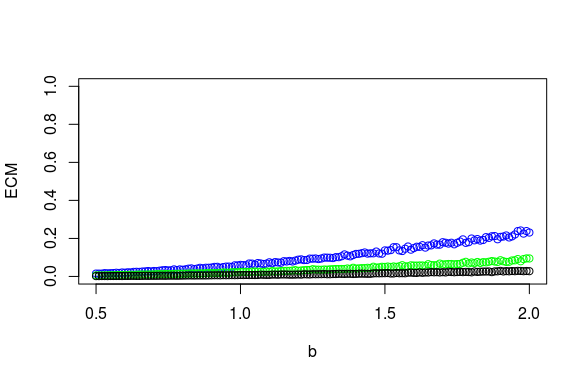
\includegraphics[scale=0.75]{ej6.png}
En este gráfico, los puntos azules representan el estimador de mediana, mientras que los verdes al de momentos y los negros al de máxima verosimilitud.
Observamos que el de máxima verosimilitud tiene menor error. Por lo tanto elegiríamos ese.

\section{Ejercicio 7}
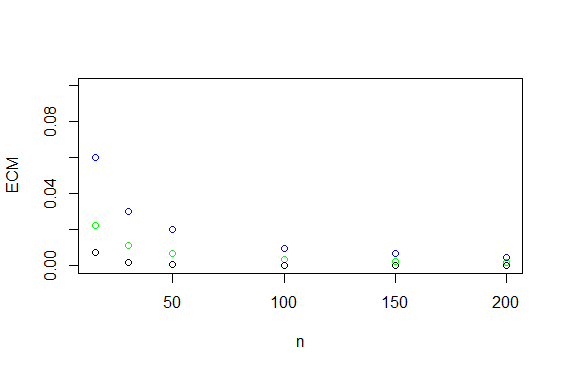
\includegraphics[scale=0.75]{ej7.png}
En este segundo gráfico, cada color representa al mismo estimador que en el Ejercicio 6.
Observamos que nuevamente el $b_{mv}$ es el que tiene menor ECM. Nos llama la atención que $b_{med}$ tenga un comportamiento tan distinto a los otros dos estimadores. Elegimos nuevamente $b_{mv}$. En todos los casos, pero particularmente en $b_{mv}$ y $b_{mom}$, observamos que el estimador se acerca al valor estimado mientras más grande es el $n$, pero se puede observar en este grafico puntualemnte, el $b_{mv}$ es el que tiene un menor ECM en los primeros 4 valores de la muestra que el $b_{mom}$. Ademas tanto el $b_{mom}$ y el $b_{mv}$ son consistentes.

\section{Ejercicio 8}
La diferencia que hay entre cada uno, al parecer el $b_{med}$ es el que se acerca mas al valor real, siendo que es uno de los valores de la muestra. Entendemos que se debe al outlayer 20.1

\newpage

\section{Ejercicio 9}
\newline

\begin{table}[h!]
\centering
\caption{Tabla comparativa}
\label{my-label}
\begin{tabular}{llll}
\hline
\multicolumn{1}{|l|}{}                  & \multicolumn{1}{l|}{\textbf{MOM}} & \multicolumn{1}{l|}{\textbf{MV}} & \multicolumn{1}{l|}{\textbf{MED}} \\ \hline
\multicolumn{1}{|l|}{\textbf{Sesgo}}    & \multicolumn{1}{l|}{0.328388}   & \multicolumn{1}{l|}{2.38277}   & \multicolumn{1}{l|}{-0.5004894}    \\ \hline
\multicolumn{1}{|l|}{\textbf{Varianza}} & \multicolumn{1}{l|}{2.857373}     & \multicolumn{1}{l|}{158.4417}    & \multicolumn{1}{l|}{0.01482475}   \\ \hline
\multicolumn{1}{|l|}{\textbf{ECM}}      & \multicolumn{1}{l|}{2.965211}     & \multicolumn{1}{l|}{164.1193}    & \multicolumn{1}{l|}{0.2653144}    \\ \hline

\end{tabular}
\end{table}

En este caso, preferimo el $b_{med}$, ya que es el que más se acerca al valor real y siendo que el que posee el menor ECM.

\end{document}
